\chapter{Negotiating researcher and participant relationships}
\label{NegotatingReseacherParticipantRelationships}
\section{Introduction}
\label{Relationships:Introduction}
Anyone who has worked with participants in sensitive contexts will know the unique challenges that arise with the role of being a researcher, carer, family member, and friend. Through a researcher's conversations and interactions, the narrative we tell is entangled and influenced by other people's narratives. Within this chapter, I describe a three year auto-ethnography that explores my path into designing in dementia and HCI research. Through two studies, I reflect on guidance into designing media and VR experiences \textit{for} and \textit{with} people living with dementia. As I recall the prior three years, there is a gradual shift from VR technology being a critical part of the research, to placing importance on the broader concerns about ethics in the community of practice. For example, how does short-term memory, need for care, orientation, and a culture of ethical 'protectionism' impact the involvement of people living with dementia in research.  This chapter covers two- and half-year engagement with a dementia café in Newcastle known as Silverline Memories. This local registered charity prides itself on its activities, organising celebrations for members' birthdays and other special occasions. With designing for creativity becoming an essential shift in design research in dementia \citep{john_killick_claire_craig_creativity_2012,morrissey_creative_2015,wallace_design-led_2013}, the potential for VR for people living with dementia may come hand-in-hand with ways to experience and express creativity. In the first study, I explore designing tailored VR experiences, which leads to an exploration of how we design for media capture of meaningful experiences to support families living with dementia.

Given the chapter is about the narrative of relationships that are formed through participatory research, I describe several stories told by my Grandma that influenced my thought process and journey through these two individual studies. These stories are about the ways in which she cared for my Grandpa, who lived with Alzheimer's, that either echoed similarities of the stories carers and dementia advocates share, or at the very least, had an impact on why I decided to approach the area of HCI and dementia. Therefore, by taking a experience-centred design approach \citep{mccarthy_technology_2007}, not only  was I required to closely work with participants to engage in open and exploratory examinations of their lived experiences, I must consider the shifting identities adopted through the research. From being a researcher, volunteer, friend, and Grandson, I explore how these identities overlap and influence one another. 

The two studies covered in this chapter were peer-reviewed and published at the CHI Conference on Human Factors in Computing Systems \citep{hodge_exploring_2018,hodge_exploring_2019}. Both papers were co-authored by Dr. Kellie Morrissey and Sandra Hastings, with additional co-authorship from Dr Madeline Balaam for the 2018 paper, and Dr Kyle Montague for the 2019 paper. While this chapter expands on the auto-ethnography data that was not used for either publications, I acknowledge that ideas and arguments in the chapter are influenced by the publications. Furthermore, section \ref{Relationships:MomentBoxes} acts as a set of design decisions that are described in a published book chapter for 'HCI and Design in the Context of Dementia \citep{hodge2020sharing} that was co-authored by Dr Kellie Morrissey who provided feedback on the paper's writing and contribution. 

\subsection{Taking a situated knowledge approach}
\label{Relationships-Intro:SituatedKnowledge}
Given the 'outsider' perspective I have within the dementia community, I drew from Kaomea \citep{kaomea_dilemmas_2001}, which describes the importance of recognising and respecting participants' views and what they share, mainly when acting as an 'outside' researcher. While someone living with dementia may describe their experiences and reflect on diagnostic stigma, I can only make sense of the experiences I may identify with as an outsider. For example, I can think about what it is like to have family or friends distance themselves from me. However, the experiences are confined only to thought, as I can never experience what a participant has said. Crucially, this does not mean I cannot be influenced by what I heard from others. By considering the experience \textit{"in the context of a past, and a future, we may give it a meaning that is more personal to us"} \citep{mccarthy_technology_2007} that may open up new questions and understandings into the area of research. Additionally, McCarthy and Wright describe how narratives are interpretations and do not mirror what \textit{'actually'} happened. As the researcher constructs the narrative, they have a responsibility to \textit{"position ourselves in the story. By expressing ourselves to others, we show something of how we feel about the experience being described and how we feel about ourselves in that experience"} \citep{mccarthy_technology_2007}. Through relfecting on the \textit{'inward'} perspective of the researcher's identity, this auto-ethnography takes a wide-angle lens \citep{ellis_heartful_2016} to consider what the research means to the \textit{'outside world'}.

\section{Learning from people living with dementia}
\label{Relationships:Learning}
In November 2016, I started my final undergraduate year in the School of Computing at Newcastle University. Given my interests in the HCI and developing technology around dementia, Dr Madeline Balaam and Dr Kellie Morrissey were suggested to supervise my final year project. Given my family history, I was interested in exploring how I could build nuanced technology for people living with dementia. My Grandpa was diagnosed with Alzheimer's in his early 50's, and my Grandma took care of him until he passed away when he was 67 (2001). I wanted to know more about the neurodegenerative condition and understand what my Grandpa and Grandma went through. My Grandpa was only around till I was five, and from those five years, I remember very little of seeing any changes in him through those years. From what I remember, he was less physical and verbal than others around him, but my memory is rather patchy and is now filled with stories from my Grandma's view instead. My Grandpa lived with dementia for about 10-15 years, but my Grandma always said the \textit{"toughest times he faced were the first few years"}. The diagnostic labelling of dementia can have a detrimental effect on those living with dementia and their social group around them. In dementia writing, this labelling is often represented as a \textit{'loss of self'} or \textit{'non-person'} or an \textit{'un-becoming of self'} \citep{fontana_alzheimers_1989,kontos_embodied_2005}. 

Often in society, the view of dementia has been criticised as a "medicalization of deviance" \citep{bond_medicalization_1992} over prioritising maintaining a sense of self. For my Grandma and others, friends and family often abandon or become almost strangers to the person living with dementia. It's common for those who have experienced dementia in some way to have experienced or heard stories of friends or family members abandon or socially exclude themselves from the person living with dementia's lives. As this social exclusion continues, this can deprive the person living with dementia of their personhood and quality of life \cite{taylor_recognition_2008}. My Grandma told me of the time when she had got 'fed up' with my Grandpa's attitude: \textit{"all he was ever doing was staying in his shed and feeling sorry for himself. I couldn't handle it anymore. I couldn't deal with seeing him like this, nor could I deal with feeling so lonely. I told him to stop feeling sorry and take a walk with me"}. The progression of dementia also has social ramifications within the family structure, as family or friends become the caregiver, and the person living with dementia becomes the care-receiver. In particular, social activity can decrease, which entails several \textit{'knock-on'} effects such as a decline in emotional well-being, and increased social isolation and depression. 

With no current cure for dementia, technology fitted how it could have improved my Grandpa's and Grandma's more quality of life. The shift from medicalisation towards the quality of life attracted research that leveraged creativity \citep{john_killick_claire_craig_creativity_2012, lazar_critical_2017} and evoked emotion \citep{morrissey_creative_2015,wallace_design-led_2013} to allow creative communication. All the readings above had clear influences from person-centred care \citep{brooker_what_2003, kitwood_towards_1992} where the person living with dementia is treated as an individual; by including the person living with dementia in the research process and acknowledging \textit{"changing individual strengths and vulnerabilities"} \citep{suijkerbuijk_active_2019}. In the area of HCI and dementia, a wide range of technology had already been considered. For example, PlayStation moved controllers to encourage group dancing \citep{morrissey_im_2016} to touch screen displays that display music, video, and photos to support general reminiscence \citep{astell_stimulating_2010}. However, one technology that had been underexamined was VR. As VR technology was growing commercially in 2016, it had its fair share of considerations on the impact on healthcare, such as treatment of PTSD, pain management and cognitive processes \citep{hoffman_virtual_2000, schultheis_application_2001, slater_sense_2013}. While several studies seemed promising, prior work did not consider the technology as an expressive and creative medium for people living with dementia. 

From the very start of my project, there was a significant difference in the work I'd be doing compared to my colleagues on my course. While many of us decided on working with different communities and groups, rarely did any of them have to fill in such an extensive ethical form to conduct their research. At the time, it didn't feel that out of place or obtrusive. Over time, as I spent time working with people living with dementia, I became conflicted over how a researcher can conduct sensitive research when following a set of ambiguous and generic principles. Comparing my ethics form to the outcome of the study didn't align at all. By expressing the study through tick boxes and linear questions, researchers have to attempt to foresee the research and what may go wrong. Filling risk assessment forms help to give the ethics reviews an indication of how the researcher would act in particular situations, but what about moments that could not be considered? Could an act of trying to 'help' end up causing harm? As Lichtner describes below:

\begin{quote}"He kept falling asleep on the chair. And when awake, tried to get out of the chair. I told him to wait and went looking for somebody to help him. At the nurses' station, the clerk said there is a risk of falling, not to let him get out of the chair. When I explained that I was not authorised to intervene, she said she isn't either but that better to intervene than to have a fall. So, I went back to the patient and thought that if I engaged him in conversation he would stop trying to get up" \citep{lichtner_everyday_2014}
\end{quote}

Lichtner discusses the difficulties of reducing their presence in the ward but found themselves either intervening or explicitly being asked to help. Acts of ambiguity are ordinary in socially-oriented research but challenge the ethical complexities of conducting research. Often, researchers are placed into an ethical dilemma, where they have no time to ask for another's advice and make a split-second decision. Similarly, they are times where I've taken an ethical' snap decision', and I have felt guilty for it. But spending time outside the field, learning by reading other people's accounts in socially-oriented research, not only normalised my decisions but helped me prepare for the next ethical dilemma to be faced. By reading other researchers acts of ambiguity in the field, many of the conflicts centred around a lack of understanding from the ethical review boards (ERBs) for the research being conducted. Perhaps, if ERB's engaged with the community, review boards would gain insight into the type of ethical practices that should be in place for that particular community. Furthermore, working with the community would also allow those affected to articulate their interests and priorities at the building block stages of the research study.

Throughout December and January 2017, I started to consider what it meant to create workshops that encouraged engagement, particularly within socially-oriented research. Guided by the network of collaborators Open Lab had, I conducted a series of workshops at a dementia café on the outskirts of Newcastle city centre. For the first workshop, I wanted to find out what participants may wish to see in a VR experience and know anything about VR. Working alongside Dr Kellie Morrissey, we set out to Silverline Memories dementia café, and I felt nervous. I felt so out of place. Apart from my experience with my Grandpa when I was a child, I had never really experienced being around people living with dementia. Kellie and I arrived at the dementia café a little earlier than Sandra (who runs Silverline Memories). Sandra came later than us with bags full of snacks and drinks for their dementia café session. As we approached the dementia cafe, it was apparent this was a community room attached to a church. We helped Sandra carry the bags into the boxed room that, while felt outdated, had its uses. On the left side was a kitchen area for volunteers and to hand out tea, coffee and biscuits throughout the session – while this was for volunteers/staff, if members walked in, no one was told to leave. Instead, volunteers would ask what they would like. They had an unlocked door opening up into the church to the very back of the kitchen, which was used for sessions when they split carers and people living with dementia into different activities. To get used to the room and distract me from the nerves, I helped set the space up seen in Fig.\ref{fig:SilverlineCommunityRoom}.

\begin{figure}
\centering
\begin{subfigure}{.5\textwidth}
  \centering
  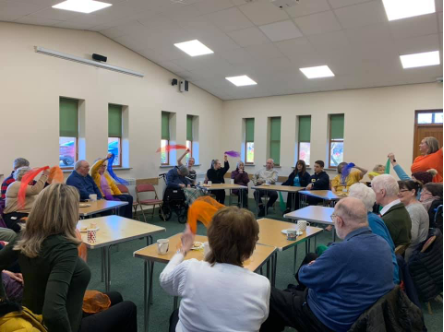
\includegraphics[width=.8\linewidth]{Images/SilverlineCommunityRoomOne.png}
  \label{fig:sub1}
\end{subfigure}%
\begin{subfigure}{.5\textwidth}
  \centering
  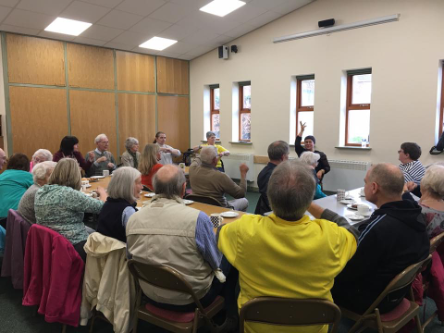
\includegraphics[width=.8\linewidth]{Images/SilverlineMemoriesCommunityRoomTwo.png}
  \label{fig:sub2}
\end{subfigure}
\caption{Silverline memories community room (taken from Silverline Memories Facebook)}
\label{fig:SilverlineCommunityRoom}
\end{figure}

 With the community room being shared across many different groups, Silverline memories had never had the chance to make space their own. Instead, you had a sense of 'home' or 'community' through the interactions with the volunteers and members. As I had set up the room, I got my notebook out, VR headset, and a recorder and consent/information sheets. As the first couple entered the café, Sandra and the other volunteers came over to them with open arms – similar for everyone who walked in on that day. They caught up, got them a cuppa tea and biscuits and got them sat down. Sandra was immediately welcoming and had created a space that focused less on the diagnosis and more on creating social interactions through creativity, music, entertainment and shared experiences. Sandra introduced the couple – Philip and Kate, to Kellie and I, and they were so appreciative and warm. They asked about the research, what we did, and showed such enthusiasm for why we were there. As I would find out in the study, the initial few minutes of signing consent, and reading information sheets and explaining the research are uncomfortable for all those involved. At that moment, it went from an informal conversation and into a formal study where two of us would be analysing and studying what was said. As we described the study, both were very happy with taking part in the conversation about the types of VR experiences they'd like to see. They were okay with quotes being used as long as they were anonymised. 

The workshop was my first experience working with people living with dementia, but more importantly, the first time I would be seen as a 'researcher'. Although looking young, and of course, getting sarcastic comments from the participants about my age and that I'm too young to be a researcher, I didn't know how to conduct myself in conversations with this new title. Each conversation felt like an interview, and there was a sense of power imbalance.  In some instances, power imbalance came from both sides, with members of Silverline Memories having been a part of the cafe for some time. Members didn't have to talk to us or take part in the study, and if they didn't, they had nothing to lose. On the other hand, Kellie and I were the only ones walking around with that title of 'researcher' who were here to interview and record participants. It was so unnatural to me, but why would it be natural? I don't start my conversations with friends or family with consent forms and placing an audio recorder on the table. Yet, the methodologies I was told to follow focused on the importance of researcher-participant relationships. 
 
From our conversation, I was surprised to see such common links with other papers I had read around HCI and dementia - people wanted an experience and 'fun' with the technology. Thomas wasn't interested if VR could help reduce care or anything focused on medicalisation, just how technology could be used as a form of entertainment. Thomas expressed Janet's passion for \textit{"listening to music and playing"} and that when she was younger, \textit{"she used to be in a choir... so it's been a big part of her"}. Regularly, the couple would explore YouTube videos looking for performances, which is why Thomas suggested a virtual theatre as he thought it'd be an \textit{"effective way of allowing her to experience something approaching live music once more"}. As our workshop ended, we had gained an overview of what may and may not work with the environments we would be creating. I then returned in a month with three different VR environments - a beach, park and a tailored Shania Twain concert hall for Janet and Thomas.
 
As I sat down writing, I felt a strain of being a 'researcher' or an 'outsider' in this perspective'. Akindes says that \textit{"through reflection, the meaning becomes visible in the process of writing"} \citep{akindes_pahalas_2001}. In this case, I'm talking about my privilege. As a white British male, I had never taken on any particular title that may place me as an 'outsider' throughout my entire life. Many of the members were warm and welcoming to myself, but I will always remain as an outsider to some degree. Although we share some aspects of experiences with all the members of Silverline Memories being from the UK, based on their stories and mine, they are drastically different. Throughout my life, I've remained in education and had the opportunity to go to university. At the same time, many of the participants I talked to discussed stories of their working-class upbringings that I had no perspective to draw upon. Therefore, I remain to question am I a good fit to research into the area of dementia. Christine Bryden discusses how by living with dementia\textit{ "[she] ha[s] complete member research status and can provide an insiders perspective"} \citep{bryden_challenging_2020}. However, while this gives Bryden an insider perspective to her own experiences and an understanding in the similarities that are present with a diagnosis with dementia, as ethnographers, \textit{"we are never fully outside or inside the "community"} \citep{naples2003feminism}. Naples argues that during research, \textit{"we negotiate and renegotiate our relationship to the community through particular and ongoing everyday interactions"} \citep{naples2003feminism}. Even if I had been part of Silverline Memories for numerous years, the addition of the 'research' title would have shifted my identity within the group. If we consider gender, race inequality, and class divisions as part of the outsider phenomenon, then we must acknowledge the \textit{"powerful role we play in shaping what can be seen"} \citep{naples2003feminism}. While as a researcher, we are not the only ones creating the academic knowledge nor can we control its effects, we must be aware that it plays an essential role during and after the research \citep{irwin_into_2006}. Whether we believe we have an outsider or an insider perspective, our research is to make changes to the research population, not ourselves. 

\section{Designing VR environments}
\label{Relationships:DesigningVR}
Over the next month of creating the VR experiences, I felt immense anxiety and stress about creating something interesting. Even though expectations may have been low from the participants, the pressure to make a well-researched project from my final year project and that I didn't want to let Sandra or the participants down was on my mind. Over that month, conversations with my Grandma consisted of sharing our experiences of dementia. While we had different understandings and experience, I realised the challenges she faced as a caregiver—mine from a research perspective and hers from a caring one. Pursuing dementia research not only was a personal endeavour from prior family history, but it also opened up conversations I had always been afraid to ask of my Grandma. Selfishly I know, but asking more about my Grandma's relationship with dementia, I thought, would give me a clearer perspective of how I may design for people living with dementia. I'm not sure if it did, but it gave me a sort of connection and empathetic feeling to the topic. I continued to be interested in the area, and during that time, I got to connect in a way to my Grandpa; I never thought I would have. Listening to my Grandma's stories about the challenges that came from his diagnosis influenced my perspective on dementia research.  The influence and relationship I have with my Grandma is a significant one in my research. While her stories painted a picture of their relationship that had its 'ups and downs', it was relatively a positive story of living with Alzheimer's. Over time, I began to realise and acknowledge that I overlooked the challenges and complexities that people with dementia may face - either the individual or carers. Only by spending more time in Silverline Memories – with other people living with dementia, would I gain a more in-depth understanding of the vastly different experiences people have had.  

With around four weeks to develop the VR environments, I enrolled in a VR online course by Udacity. With VR development being relatively new and not an area the university specialised in, I contacted the online course representative at Udacity to consider myself for a scholarship for their VR course. In early February, they got back to me and found the study of personalised VR for people living with dementia "innovative" and "novel" to the area. They sent me an online access code, and throughout February, I started to juggle learning VR game development with the rest of my university modules. The course gave me invaluable experience in building VR environments in Unity (a game engine). However, what it didn't describe was the importance of the particular placement of objects within the environment. For this project, I applied Mike Alger's \citep{alger_visual_2015} concept of content zones that I describe in fig.\ref{fig:ContentZone} that helped reduce risks of sickness or disorientation and improve the individuals' overall experience. 

\begin{figure}
\centering
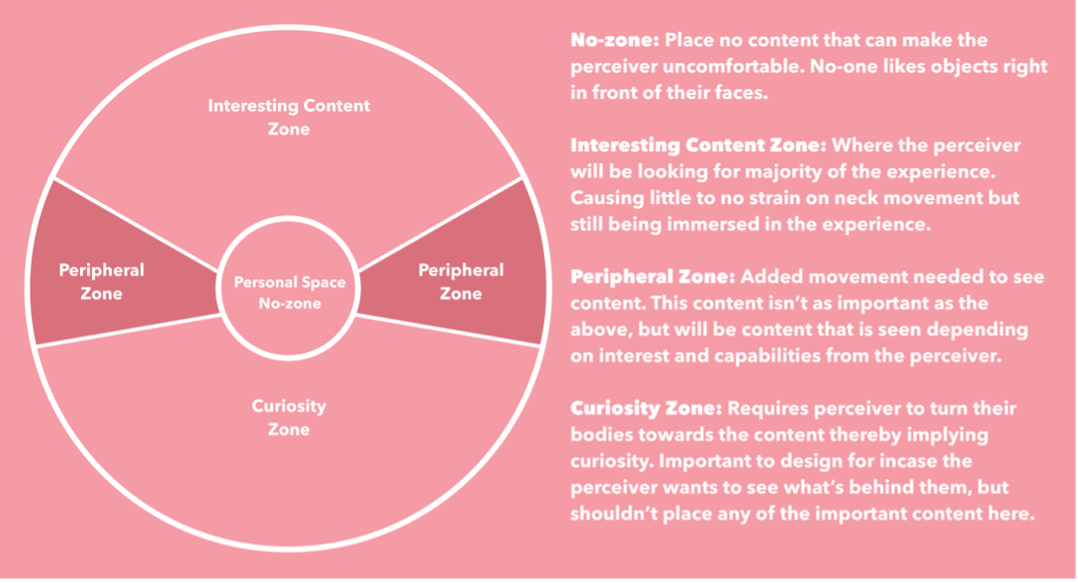
\includegraphics[width=.8\linewidth]{Images/ContentZones.png}
\caption{Content zones in VR}
\label{fig:ContentZone}
\end{figure}



\section{Moment Boxes}
\label{Relationships:MomentBoxes}